\documentclass[12pt]{article}

\usepackage[a4paper,margin=1in]{geometry}
\usepackage{graphicx}
\usepackage{amsmath}
\usepackage{booktabs}
\usepackage{float}
\usepackage{hyperref}

\title{\textbf{Task-2 SubTask-1}\Road Segmentation using Deep Learning Architectures}
\author{Tilak Asodariya}

\begin{document}

\section{Introduction}

Semantic segmentation aims to classify every pixel in an image into predefined categories. In road segmentation, the objective is to accurately identify road pixels from aerial imagery.

Road extraction is useful in numerous applications such as:

\begin{itemize}
\item Geographic Information Systems (GIS)
\item Autonomous Navigation
\item Urban Planning
\item Infrastructure Monitoring
\end{itemize}

Recent advances in deep learning have significantly improved segmentation performance. Encoder-decoder architectures such as U-Net have become widely used because they preserve spatial information while learning high-level semantic representations.

This project investigates the effectiveness of several segmentation architectures on the Massachusetts Roads Dataset and compares their performance under identical preprocessing and training conditions.

\section{Dataset}

The Massachusetts Roads Dataset was used for all experiments.

The dataset consists of:

\begin{itemize}
\item Training Images
\item Validation Images
\item Test Images
\item Corresponding Binary Road Masks
\end{itemize}

The original dataset is distributed in TIFF format and contains aerial imagery with manually annotated road masks.

A major challenge in this dataset is class imbalance. Road pixels occupy only a small fraction of each image, while most pixels belong to the background class.

\section{Data Preprocessing}

A preprocessing pipeline was developed before training.

The following operations were performed:

\begin{enumerate}
\item Resize all images to 512$\times$512.
\item Resize masks to 512$\times$512 using nearest-neighbor interpolation.
\item Convert all TIFF images and masks into PNG format.
\item Store processed data in dedicated train, validation, and test folders.
\end{enumerate}

Lanczos interpolation was used for images while nearest-neighbor interpolation was used for masks to preserve binary labels.

The processed dataset was then used for all experiments.

\section{Loss Function}

Road segmentation suffers from severe class imbalance because background pixels dominate the image.

To address this issue, a combination of Binary Cross Entropy (BCE) Loss and Dice Loss was used.

\begin{equation}
L = L_{BCE} + L_{Dice}
\end{equation}

BCE Loss provides stable pixel-wise supervision while Dice Loss directly optimizes overlap between predicted and ground-truth masks.

Dice coefficient is defined as:

\begin{equation}
Dice = \frac{2|P \cap G|}{|P| + |G|}
\end{equation}

where:

\begin{itemize}
\item $P$ = Predicted Mask
\item $G$ = Ground Truth Mask
\end{itemize}

This combination was selected because BCE alone tends to favor background prediction while Dice Loss directly addresses segmentation overlap.

\section{Evaluation Metrics}

Two evaluation metrics were used.

\subsection{Dice Score}

Dice Score measures overlap between predicted and ground-truth masks.

Higher values indicate better segmentation quality.

\subsection{Intersection over Union (IoU)}

IoU is defined as:

\begin{equation}
IoU = \frac{|P \cap G|}{|P \cup G|}
\end{equation}

IoU provides a stricter evaluation criterion and is commonly used in segmentation benchmarks.

\section{Baseline U-Net}

The baseline model uses a standard U-Net architecture.

The encoder consists of four stages:

\begin{center}
64 $\rightarrow$ 128 $\rightarrow$ 256 $\rightarrow$ 512
\end{center}

Skip connections transfer spatial information from encoder layers to decoder layers, allowing accurate reconstruction of road structures.

Training configuration:

\begin{itemize}
\item Input Size: 512$\times$512
\item Batch Size: 8
\item Learning Rate: 1e-4
\item Epochs: 10
\item Optimizer: Adam
\item Loss Function: BCE + Dice Loss
\end{itemize}

\section{Architectural Improvements}

To investigate whether more advanced architectures could improve segmentation performance, three additional models were evaluated.

\subsection{ResNet34 U-Net}

The standard encoder was replaced with a pretrained ResNet34 backbone initialized using ImageNet weights.

Motivation:

\begin{itemize}
\item Faster convergence.
\item Better feature extraction.
\item Improved transfer learning.
\end{itemize}

Potential improvements:

\begin{itemize}
\item More training epochs.
\item Stronger data augmentation.
\item Larger backbones such as ResNet50 or EfficientNet.
\end{itemize}

\subsection{DeepLabV3+}

DeepLabV3+ introduces Atrous Spatial Pyramid Pooling (ASPP) to capture contextual information at multiple scales.

Motivation:

\begin{itemize}
\item Better global context understanding.
\item Improved detection of long road structures.
\item Multi-scale feature extraction.
\end{itemize}

Potential improvements:

\begin{itemize}
\item Higher learning rates.
\item Longer training schedules.
\item Deeper encoder backbones.
\end{itemize}

\subsection{SegFormer}

SegFormer is a transformer-based semantic segmentation architecture.

Motivation:

\begin{itemize}
\item Global attention mechanisms.
\item Better modeling of long-range dependencies.
\item Strong multi-scale feature aggregation.
\end{itemize}

Potential improvements:

\begin{itemize}
\item Larger transformer variants.
\item Learning rate warmup.
\item Extensive augmentation.
\item Larger datasets.
\end{itemize}

\section{Results}

The following results were obtained on the test set.

\begin{table}[H]
\centering
\caption{Performance Comparison}
\begin{tabular}{lcc}
\toprule
Model & Dice Score & IoU \\
\midrule
U-Net & 0.7245 & 0.5690 \\
ResNet34 U-Net & 0.7180 & 0.5612 \\
DeepLabV3+ & 0.6093 & 0.4383 \\
SegFormer & 0.5726 & 0.4012 \\
\bottomrule
\end{tabular}
\end{table}

The baseline U-Net achieved the highest Dice Score and IoU among all evaluated architectures.

\section{Training Curves}

Figure \ref{fig:loss} shows the training and validation loss curves for the baseline U-Net.

\begin{figure}[H]
\centering

\includegraphics[width=0.9\textwidth]{loss.png}
\caption{Training and Validation Loss}
\label{fig:loss}
\end{figure}

The loss curves decrease steadily without signs of divergence or overfitting.

Figure \ref{fig:metric} shows the progression of Dice Score and IoU during training.

\begin{figure}[H]
\centering
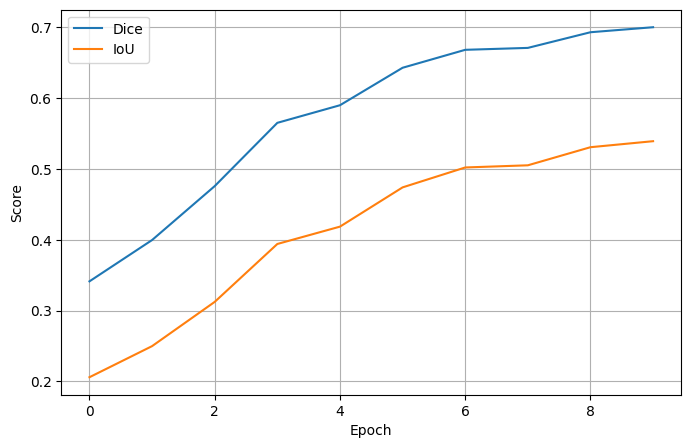
\includegraphics[width=0.9\textwidth]{metric.png}
\caption{Dice Score and IoU Progression}
\label{fig:metric}
\end{figure}

Both metrics improve consistently throughout training, demonstrating stable optimization.

\section{Qualitative Results}

Sample predictions from the baseline U-Net are shown in Figure \ref{fig:preds}.

\begin{figure}[H]
\centering
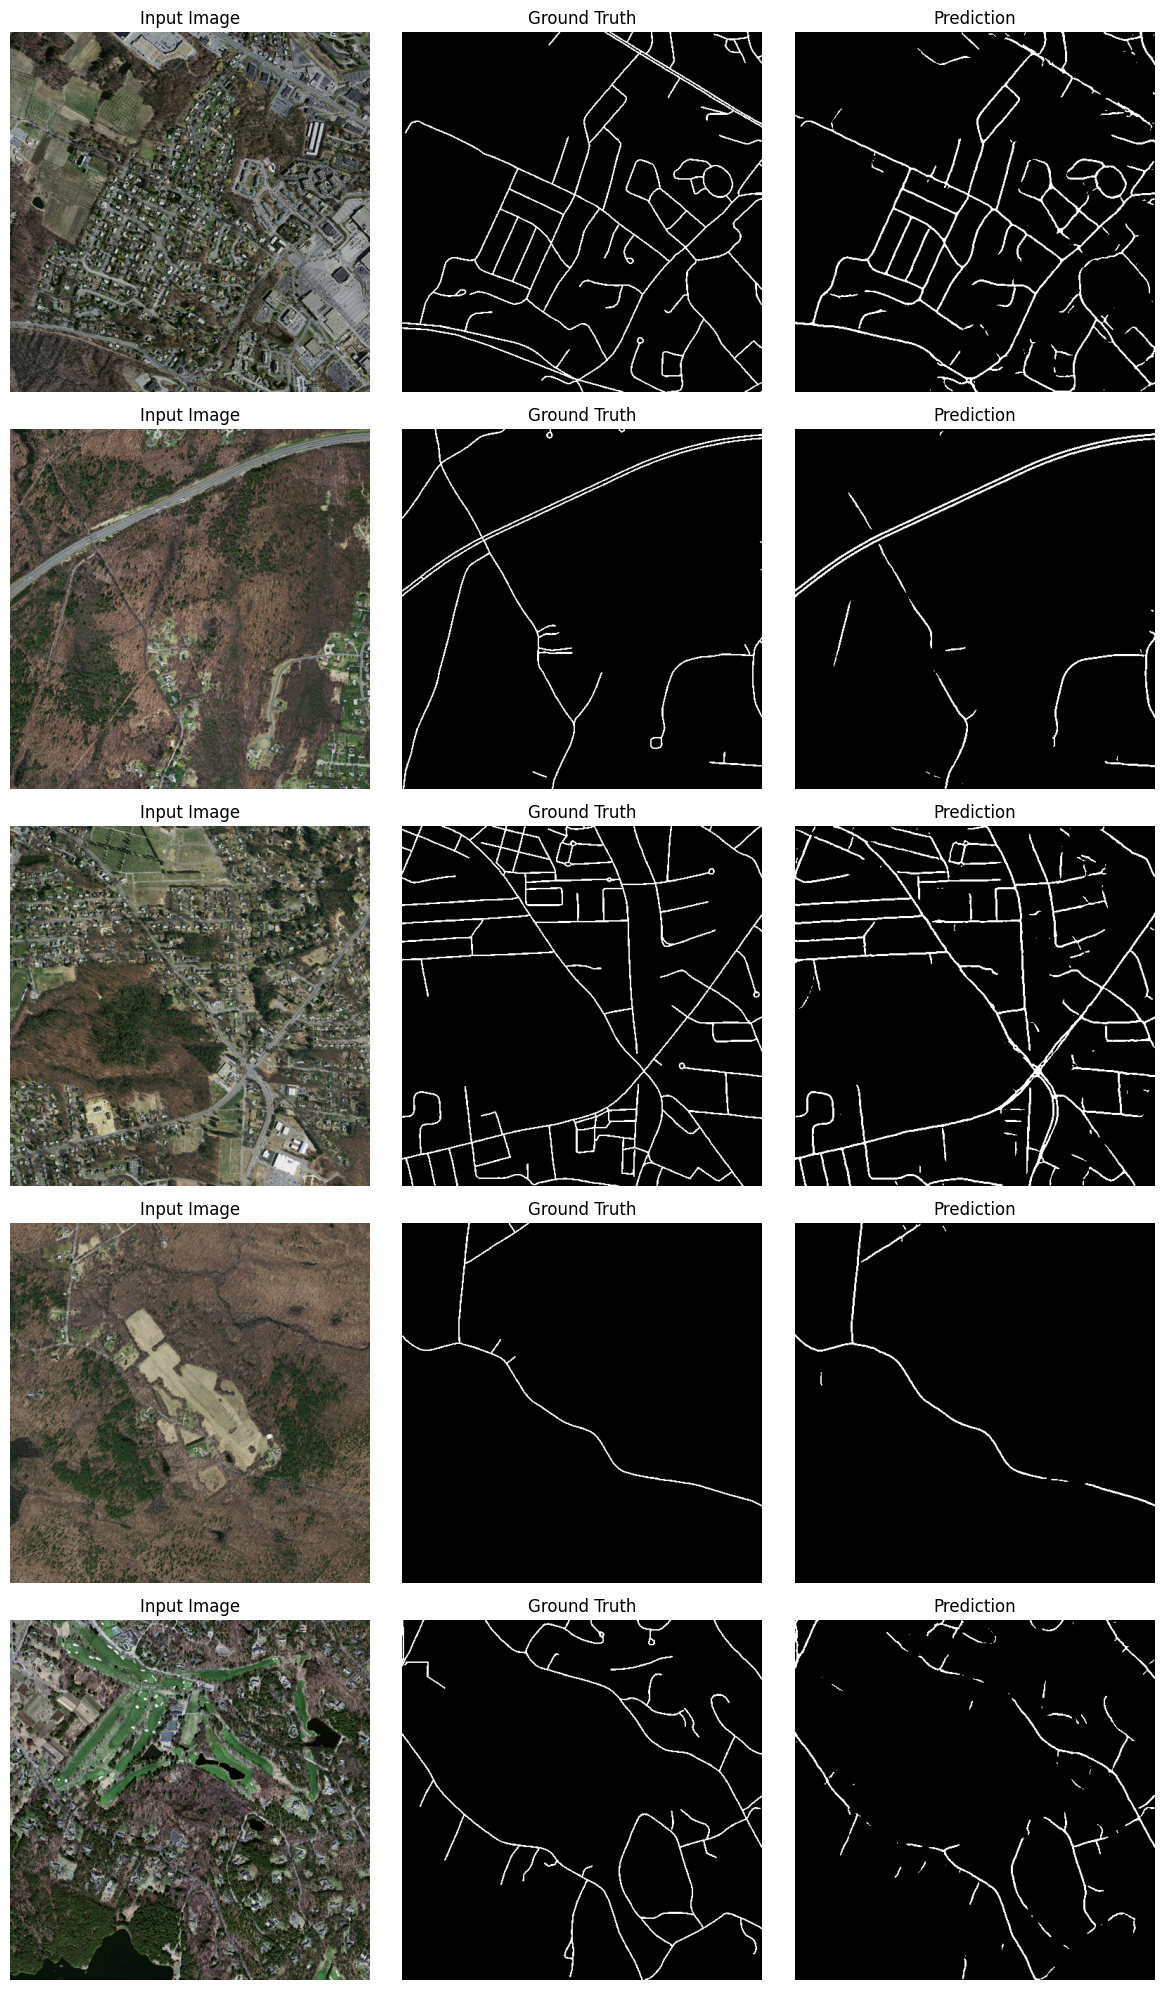
\includegraphics[width=0.5\textwidth]{preds.png}
\caption{Sample Road Segmentation Predictions}
\label{fig:preds}
\end{figure}

The model successfully captures major road structures and intersections. Most segmentation errors occur on thin residential roads and small road branches.

\section{Discussion}

The baseline U-Net achieved the strongest overall performance despite being the simplest architecture evaluated.

The ResNet34 U-Net converged faster due to transfer learning but produced nearly identical final performance.

DeepLabV3+ showed steady improvement when trained for additional epochs but remained significantly below the baseline.

SegFormer demonstrated the weakest performance under the chosen training budget. Transformer-based models generally require larger datasets and more extensive hyperparameter tuning to realize their full potential.

These findings suggest that the Massachusetts Roads Dataset favors architectures that preserve fine spatial details through skip connections.

\section{Conclusion}

This project investigated multiple deep learning architectures for road segmentation using the Massachusetts Roads Dataset.

The baseline U-Net achieved the best overall performance:

\begin{itemize}
\item Dice Score: 0.7245
\item IoU: 0.5690
\end{itemize}

Although more advanced architectures such as ResNet34 U-Net, DeepLabV3+, and SegFormer were evaluated, none surpassed the baseline model under identical training conditions.

The results demonstrate that a carefully trained U-Net combined with BCE and Dice Loss remains highly effective for aerial road segmentation tasks.

\end{document}
